\documentclass{article}
\usepackage[utf8]{inputenc}
\usepackage[T1]{fontenc}
\usepackage[french]{babel}
\usepackage{graphicx}
\usepackage{listings}
\usepackage{color}
\usepackage{geometry}
\usepackage{array}
\usepackage{hyperref}
\geometry{hmargin=2.5cm,vmargin=3cm}
\definecolor{dkgreen}{rgb}{0,0.6,0}
\definecolor{gray}{rgb}{0.5,0.5,0.5}
\definecolor{mauve}{rgb}{0.58,0,0.82}
\hyphenation{GitHub}

\lstset{frame=tb,
  language=Java,
  aboveskip=3mm,
  belowskip=3mm,
  showstringspaces=false,
  columns=flexible,
  basicstyle={\small\ttfamily},
  numbers=none,
  numberstyle=\tiny\color{gray},
  keywordstyle=\color{blue},
  commentstyle=\color{dkgreen},
  stringstyle=\color{mauve},
  breaklines=true,
  breakatwhitespace=true,
  tabsize=3
}

\date{\today}
\author{Tarik Atlaoui \\ Nicolas Peugnet \\ Kimmeng Ly \\ Max Eliet}

\begin{document}


\begin{titlepage}
	\enlargethispage{2cm}
	\newcommand{\HRule}{\rule{\linewidth}{0.5mm}}
	\center
	\textsc{\LARGE
	Rapport PSAR 
	} \\[1cm]
	\HRule \\[0.4cm]
	{ \huge \bfseries API générique pour le développement d'applications réparties \\[0.15cm] }
	\HRule \\[4cm]
	\large{Tarik Atlaoui \\[3mm] Nicolas Peugnet \\[3mm] Kimmeng Ly \\[3mm] Max Eliet} \\[3cm]
	08 Juin 2020 \\[3cm]
	\hfill 
\includegraphics[width=5cm]{logoSU.jpg}
\end{titlepage}

	\newpage
	\pagenumbering{arabic}
	\tableofcontents
	\newpage
		\section{Introduction}
			\subsection{Les applications réparties}
			\large{ Avant de commencer, il est important de définir ce qu’est une application répartie. Dans notre cas, nous pouvons voir une application répartie comme un ensemble d’entités logicielles, de composants qui peuvent être développés dans différents langages de programmation, s’exécutant sur plusieurs sites et qui sont reliés entre eux par une interface ou un réseau de communication.}
			\subsection{Les difficultés à programmer une application répartie}
			\large { Aujourd’hui la programmation d’applications réparties est devenue une réalité du monde informatique, cette forme de programmation permet d'augmenter la disponibilité des applications et de diminuer leur temps d'exécution. Cependant, réaliser une application répartie reste une tâche délicate. En effet, nous devons prendre en compte la maintenabilité et la réutilisabilité des programmes. De plus, les accès concurrents peuvent créer des erreurs et des sources d'incohérence. C’est pourquoi il est très important de montrer que ces programmes fonctionnent bien avec des tests unitaires tout en respectant le cahier des charges.}
		\section{Méthode de développement}
			\subsection{API réelle : avantages/inconvénients et exemple (MPI ou autre)}
			%RESTE A COMPLETER ICI
			L'API de MPI est avant tout une norme pour le passage de messages entre différents ordinateurs ou au sein d'un même ordinateur.
			Elle est énormément utilisée pour la communication sur des architectures distribuées.
			Dans notre cas, elle s'est révélée extrêmement intéressante car MPI a été implémentée sur presque toutes les architectures ainsi elle 
			a été adaptée pour chacune de la façon la plus optimale. Cependant les tests et le debug sur celle-ci restent difficiles dû a l'impossibilité 
			d'avoir un contrôle sur les évenements qui apparaissent, contrairement à PeerSim.
			
			\subsection{API simulation à évenements discrets :avantages/inconvénients et exemple(PeerSim ou autre)}
				Qu'entend-on par \textit{simulation à événements discrets}? C'est une simulation dont le temps évolue seulement lorsqu'un événement survient sur un noeud, et donc de même l'état du système ne peut être modifié qu'à ces moments là.

				On distingue donc deux entités : les noeuds, et les événements qui sont caractérisés par une date de délivrance, un noeud destinataire, et des données.

				Les principaux avantages d'un tel type de simulation sont : son déterminisme et donc une capacité à reproduire des bugs, et une charge de calcul réduite aux événements qu'on décide de simuler. Toutefois, il faut savoir trouver un équilibre entre une simulation trop simpliste et une simulation trop précise ralentie par trop d'événements.

				Dans notre cas, nous nous sommes dirigés vers PeerSim comme simulateur à événements discrets, car il est codé en Java et possède une API relativement simple d'utilisation.

				PeerSim est utilisé pour créer des nœuds et simuler une architecture pair-à-pair en générant des protocoles et des événements qui sont définis par l'utilisateur. Une éxécution est toujours ce qui permet d'accélérer le débug d'une application répartie avant son déploiement ou de reproduire une séquence d'événements qui a provoqué un bug sur une application déja existante.

			
			\subsection{Aperçu de l'implémentation d'un anneau avec les deux API}
                
            \vspace*{5mm}

                {\bfseries Implémentation en MPI}
				\begin{lstlisting}
public class RingMpi {

	public static void main(String[] args) {
			MPI.Init(args);
			Comm comm = MPI.COMM_WORLD;
			int size = comm.getSize();
			int rank = comm.getRank();
			int neighbour = (rank + 1) % size;
			int hellotag = 1;
			Integer msg = 0;
            Status status;
            
			if (rank == 0) {
				comm.send(msg, 0, MPI.INT, neighbour, hellotag);
				status = comm.recv(msg, 0, MPI.INT, MPI.ANY_SOURCE, hellotag);
			} else {
				status = comm.recv(msg, 0, MPI.INT, MPI.ANY_SOURCE, hellotag);
				comm.send(msg, 0, MPI.INT, neighbour, hellotag);
            }
            
			System.out.println(rank + " Received hello from " + status.getSource());
			MPI.Finalize();
		}
	}
}
                \end{lstlisting}
                \newpage
				{\bfseries Implémentation en PeerSim}
				\begin{lstlisting}
public class HelloProtocol implements EDProtocol {
	//Declarations d'attributs et fonctions retirees pour la clarte du code
	...
	//Un noeud souhaite faire sa diffusion du message a son voisin
	public void direVoisin(Node host) {
		Transport tr= (Transport) host.getProtocol(pid_transport);
		Node dest=Network.get((int) ((host.getID()+1)%Network.size()));
		Message mess= new Message(host.getID(),(host.getID()+1)%Network.size(),my_pid, new ArrayList<>(myList));
		tr.send(host, dest, mess, my_pid);

		deja_dit_voisin=true;
	}

	//Traitement a effectuer lorsqu'on recoit un HelloMessage
	private void receiveHelloMessage(Node host, HelloMessage mess) {
		System.out.println("Noeud "+ host.getID() + " : a recu Hello de "+mess.getIdsrc()+ " sa liste = "+mess.getInfo());
		if(!deja_dit_voisin) {
			direVoisin(host);
		}
	}
}
                \end{lstlisting}
                \vspace*{5mm}

		\section{Motivation et objectif global}
			\subsection{API générique : avantages, modèle de programmation(ici événementiel)}
				Le but de notre projet est de produire une API générique sur un modèle de programmation événementielle afin de faciliter le développement de futures applications réparties, en permettant de s'abstraire du support d'éxécution au niveau du code métier. \par
Pouvoir éxécuter le même code métier aussi bien sur une plateforme réelle que sur un simulateur permet au développeur d'une application répartie de passer de l'un à l'autre, sans risquer d'en  modifier son comportement en adaptant le code. \newline Il peut donc profiter des avantages d'un simulateur, comme la vision globale du système et le déterminisme des séquences d'éxécution  sans crainte d'y introduire de nouveaux bugs. \par
 
			\newpage
			\subsection{Aperçu de l'implémentation d'un anneau avec l'API générique}
				\begin{lstlisting}
public class ExampleNodeProcess extends NodeProcess {

	public static class ExampleMessage extends Message{
		private static final long serialVersionUID = 1L;
		public String content;
		public ExampleMessage(int src, int dest, String content) {
			super(src, dest);
			this.content = content;
		}
	}

	@MessageHandler
	public void processExampleMessage(ExampleMessage message) {
		int host = infra.getId();
		System.out.printf(
			"%d Received '%s' from %d\n",
			host, message.content, message.getIdsrc()
		);
		if (host != 0) {
			int dest = (host + 1) % infra.size();
			infra.send(new ExampleMessage(infra.getId(), dest, "bonjour"));
		}
		infra.exit();
	}

	@Override
	public void init(String[] args) {
		if (infra.getId() == 0) {
			infra.send(new ExampleMessage(infra.getId(), 1, "bonjour"));
		}
	}
}
				\end{lstlisting}
		\section{Les étapes de réalisation}
			
			\subsection{Répartition des tâches}
			\begin{tabular}{|c|c|c|}
				\hline
				Tâche & Date d'échéance & Fait par\\[1mm]
				\hline
		  		Se familiariser avec MPI et Peersim & 17/02 & Tous\\[1mm]
				\hline
				Proposer une API générique & 24/02 & Tous\\[1mm]
				\hline
				Implanter l'API pour MPI et pour PeerSim & 02/03 & Tous \\[1mm]
				\hline
				Créer une classe abstraite Message & 09/03 & Tous\\[1mm]
				\hline
				Unifier le lancement de l'application & 09/03 & Tous\\[1mm]
				\hline
				Rédiger le carnet de bord & 16/03 & Tous\\[1mm]
				\hline
				Rédiger le pre-rapport & 23/03 & Tous\\[1mm]
				\hline 
				Implanter l'aiguillage automatique des messages & 23/03 & Tous\\[1mm]
				\hline
				Ajouter la fonctionnalité de description de scenario & 30/03 & Tous\\[1mm]
				\hline
				Ajouter des fonctionnalités de wait/notify & 20/04 & Tous\\[1mm]
				\hline 
				Rédiger le rapport final & 08/06 & Tous\\[1mm]
				\hline
				Soutenance finale & 11/06 & Tous\\[1mm]
				\hline
			\end{tabular}			
			\newpage			
			\subsection{Définition API générique}
			\subsection*{API Peersim}
			\vspace{5mm}
			\hspace*{-2.2cm} 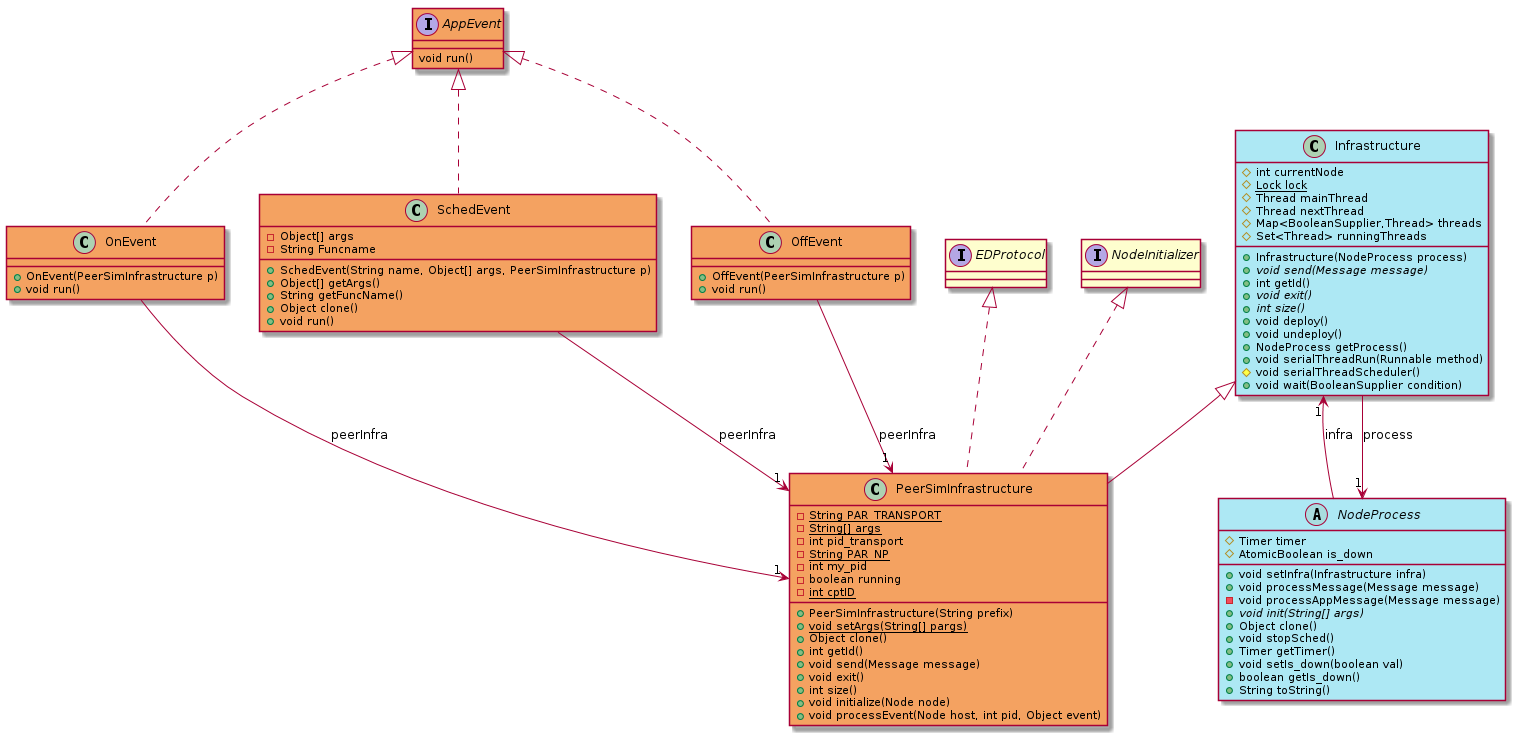
\includegraphics[width=20cm]{uml/uml_peersim_1.png}

			\vspace{20mm}
			\hspace*{-2.2cm} 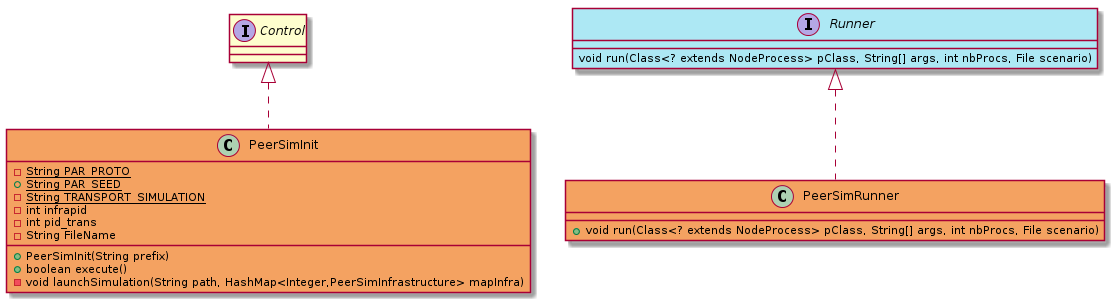
\includegraphics[width=20cm]{uml/uml_peersim_2.png}

			\newpage
			\subsection*{API MPI}
			\hspace*{-2.2cm} 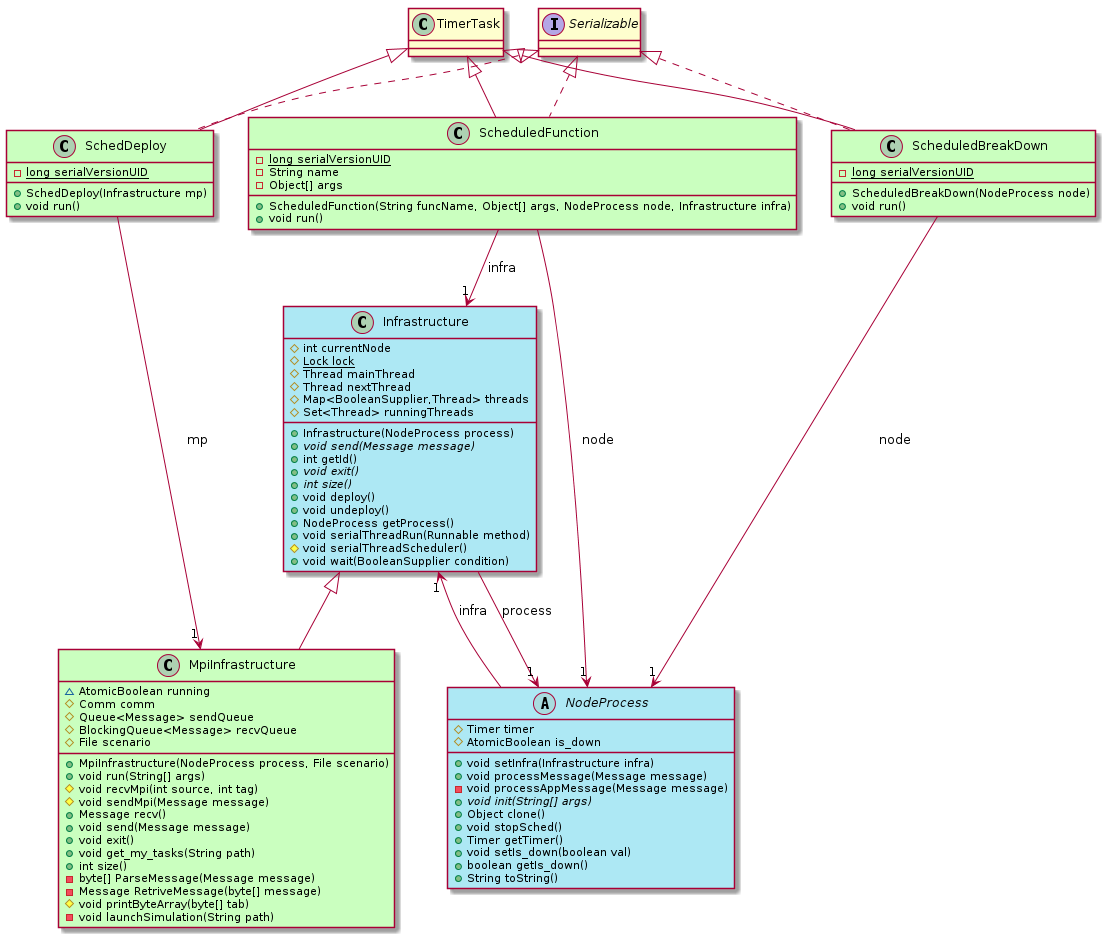
\includegraphics[width=20cm]{uml/uml_mpi_1.png}

			\vspace{5mm}
			\hspace*{-2.2cm} 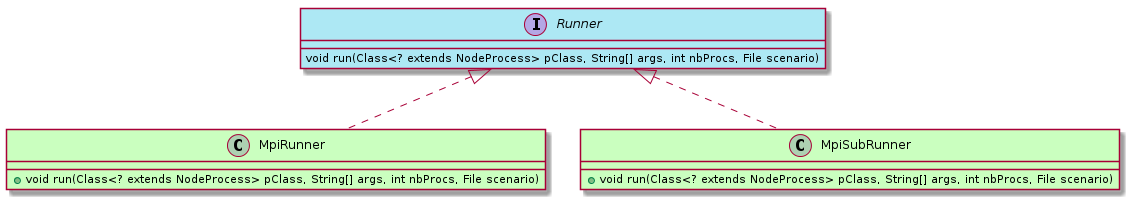
\includegraphics[width=20cm]{uml/uml_mpi_2.png}

			\newpage
			\subsection*{Main/Exécution : Ppi}
			\vspace{3mm}
			\hspace*{-2.3cm} 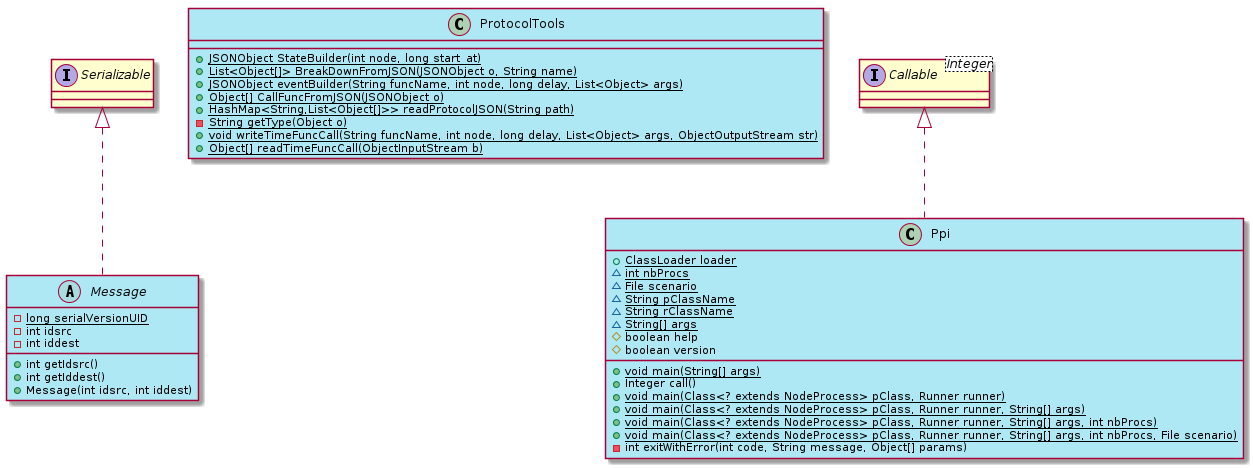
\includegraphics[width=20cm]{uml/uml_main.png}

			\vspace{20mm}
			Nous avons commencé par définir une classe abstraite Infrastructure qui contient toutes les méthodes que nos deux API (MPI et PeerSim) devront implanter et une classe abstraite NodeProcess qui est en lien direct avec Infrastructure.
			\newline
			Le lancement de ces deux applications est complètement différent, c’est pourquoi il est primordial que les deux lancements soient unifiés pour permettre un développement plus rapide et sûr. Pour remédier à cette situation, notre solution consiste à créer une interface Runner qui permet d’instancier les exécutions des deux API avec les mêmes arguments. Il suffit donc d’instancier MPIRunner et/ou PeerSimRunner avec en argument le nom de la classe qui hérite NodeProcess, le nom de la classe du Runner et (facultatifs) le nombre de processus ainsi qu’un scénario.			

			\newpage
			\subsection{Définitions des primitives offertes et explication}
			\begin{lstlisting}
			public void start();
			\end{lstlisting}
			La primitive start  doit etre redéfinie par l'utilisateur et permet de définir le code à éxécuter par le processus lors de son lancement.
			\vspace*{2.5mm}

			\begin{lstlisting}
			public void processMessage(Message message);
			\end{lstlisting}
			De même pour processMessage qui permet  de définir le comportement du processus lors de la réception d'un message.
			\vspace*{2.5mm}

			\begin{lstlisting}
			abstract class Message implements Serializable
			\end{lstlisting}
			Message est la classe définie afin de permettre une abstraction du traitement des messages et doit etre étendue par l'utilisateur.
			\vspace*{3mm}

			\begin{lstlisting}
			public void serialThreadRun(Runnable method);
			\end{lstlisting}
			Exécuter un nouveau thread qui démarrera immédiatement. 
			Le thread courrant se met en attente jusqu'à la fin d l'exécution de ce dernier ou qu'il se met en attente avant de poursuivre son exécution.
			\vspace*{3mm}

			\begin{lstlisting}
			protected void serialThreadScheduler();
			\end{lstlisting}
			Ordonnanceur qui parcourt les serialThreads en attente et les réveille s'ils peuvent continuer.
			\vspace*{3mm}

			\begin{lstlisting}
			public void wait(BooleanSupplier condition);
			\end{lstlisting}
			Cette primitive wait met le processus appelant en attente jusqu'à que la condition soit vérifiée.
			La condition doit etre un lambda retournant un booléen.
			\vspace*{3mm}

			\begin{lstlisting}
			public class Ppi
			//utilisation
			Ppi.main(new String[] {NodeProcess.class.getName(),Runner.class.getName()});
			\end{lstlisting}
			La class Ppi est le main de notre application, elle permet d'executer le code utilisateur en MPI ou en PeerSim.

			\subsection{Implantation vers MPI}
			Pour l'implantation de l'adapteur permettant d'utiliser MPI nous avons commencé par implanter un algorithme simple en utilisant cette dernière.
			Une fois que nous avons compris comment MPI fonctionne, nous avons étendu la classe Infranstructure qui représente l'abstraction des deux adapteurs implantés, pour MPI la classes MpiInfrastructure nous permet de communiquer avec MPI en ajoutant  une couche sur les primitives de MPI.
			Nous avons, cependant, dû ajouter une boucle  afin d'adapter le fonctionnement de MPI à celui de PeerSim.
			\subsection{Implantation vers PeerSim}
			Dans le cas de PeerSim, l'implantation de notre API consistait principalement à effectuer un Adapter avec l'API déjà existante de PeerSim, et donc la part la plus importante du travail était de comprendre le fonctionnement des quelques classes de PeerSim nécessaires pour faire le lien entre les deux API. Il a aussi fallu adapter certaines de nos classes pour PeerSim, par exemple rendre notre NodeProcess clonable. 
			\subsection{API pour un scenario}
			L'utilisateur aura aussi accès à une API permettant de décrire un scenario où il devra spécifier les méthodes qui devront être appeler à un temps donné ou encore 
			la panne d'un nœud. 
			\newline
			Si pour Peersim, elle utilise la procédure d'ajout d'événement et ainsi l'évènement est déclenché à la bonne date.
			\newline
			Pour Mpi nous avons utilisé la class Timer de java afin d'avoir pour chaque processus Mpi un démon qui exécutera l'évènement spécifié, les évènements peuvent cependant avoir un décalage.
			\newline
			En premier lieu, chaque évènement est dépendant de l'horloge du processus sur lequel il va être exécuté ou plus précisément l'heure à laquelle ce dernier va démarrer car chaque processus reçoit le fichier de spécification du scénario et y prend que les évênements qui le concernent.
			\newline
			Dans un second temps, la class Timer n'utilise qu'un seul Thread et par conséquent si deux évènements sont trop proches, le second évènement va attendre la fin de l'exécution du premier pour s'exécuter.

			\subsection{Fonction wait dans l'infrastructure}	
			Nous avons également implanté une primitive \textbf{wait} dans notre infrastructure. Cette primitive offre à l'utilisateur la possiblité de mettre en attente un ou plusieurs noeuds sur une condition précise.
			Les noeuds en attente reprennent leur exécution quand la condition passé en argument devient vraie.
			\newline
			\newline
			Un exemple d'utilisation de la primitive \textbf{wait} est d'afficher une information sur la sortie standard seulement
			après la réception d'un nombre N de message : 
			\begin{lstlisting}
			   public class WaitTest extends NodeProcess {
				   public static class ExampleMessage extends Message {
					   private static final long serialVersionUID = 1L;
					   private String s;
					
					   public ExampleMessage(int src, int dest, String s) {
						   super(src, dest);
						   this.s = s;
					   }
			   
					   public String getS() {
						   return s;
					   }
				   }
				   
				   private final int N = 2;
				   private int msgReceived = 0;
						   
				   public void helloN(){
					   try {
						   infra.wait( () -> msgReceived >= N );
						   System.out.println(infra.getId()+" Hello !");
					   } catch (InterruptedException e) {
						   System.out.println(infra.getId()+" Interrupted while waiting !");
					   }
				   }
				   
				   @MessageHandler
				   public void processExampleMessage(ExampleMessage message) {
					   int host = infra.getId();
					   System.out.printf("%d Received '%s' from %d.\n", host, message.getS(), message.getIdsrc());
					   msgReceived++;
					   int dest = (host + 1) % infra.size();
					   
					   if (host != 0 && msgReceived == 1) {
						   infra.send(new ExampleMessage(infra.getId(), dest, "hello"));
						   if(host==2) helloN();
					   } else {
						   infra.send(new ExampleMessage(infra.getId(), dest, "hello"));
						   infra.exit();
					   }
				   }
			   
				   @Override
				   public void init(String[] args) {
					   if (infra.getId() == 0) {
						   infra.send(new ExampleMessage(infra.getId(), 1, "hello"));
					   }
				   }
			   
				   @Test
				   public void MpiAnnotatedProcessTest() {
					   Assume.assumeTrue(Environment.mpirunExist());
					   Ppi.main(this.getClass(), new MpiRunner());
					   assertTrue(true);
				   }
			   
				   @Test
				   public void PeersimWaitNotifyTest() {
					   Ppi.main(this.getClass(), new PeerSimRunner());
					   assertTrue(true);
				   }
			   }
			\end{lstlisting}
			
			
			\subsection{Tests plus poussés des invariants}
			\subsection{Test d'exclusion mutuelle}
			\subsection{Scénario de panne}
		
		\newpage
		\section{Prise en main de notre API}

		\subsection{Programmer un algorithme}
		Pour programmer un algorithme à l'aide de Ppi il faut créer une classe qui étend la classe abstraite \lstinline{NodeProcess}. Par la suite l'ensemble des méthodes disponible seront accessibles par l'intermédiaire de la propriété \lstinline{infra}.

		\subsubsection{Etendre le classe \lstinline{NodeProcess}}
		La classe abstraite \lstinline{NodeProcess} contient une methode abstraite \lstinline{init}
		qu'il est nécessaire de redéfinir dans votre classe :
		\begin{lstlisting}
public void init(String[] args)
		\end{lstlisting}
		Cette méthode permet d'initialiser chaque processus à l'aide des arguments qui lui sont
		passés en paramètre. Elle peut être utile comme point de départ d'un algorithme où bien
		simplement pour le paramètrer.
		L'étape suivante sera de créer les différentes classes de message nécessaires au bon
		fonctionnement de votre algorithme.

		\subsubsection{Créer des classes de message}
		Chaque classe de message doit étendre la classe \lstinline{Message} et l'ensemble de son
		contenu doit être \lstinline{Serializable}. De cette manière il sera possible de les envoyer
		via Ppi et de les réceptionner à l'aide de gestionnaires de messages. Il est conseillé de
		créer une classe par type de message applicatif et ainsi de créer un gestionnaire par type
		de message.

		\subsubsection{Définir des gestionnaires de messages}
		Pour définir un gestionnaire de message, rien de plus simple. Ajoutez à votre classe
		héritant de \lstinline{NodeProcess} une fonction pernant en paramètre un objet d'une des
		classes de message que vous venez de définir et ajoutez-y l'annotation
		\lstinline{@MessageHandler} :
		\begin{lstlisting}
@MessageHandler
public void handlerTestMessage(TestMessage msg) {}
		\end{lstlisting}

		Il ne doit y avoir qu'un seul gestionnaire de message par classe de message, sinon le
		premier trouvé sera choisi par Ppi.

		\subsubsection{Méthodes à dispositions}
		Les méthodes mises à disposition par Ppi correspondent à l'ensemble des fonctions publiques
		de la classe abstraite \lstinline{Infrastructure} dont une instance est accessible via la
		propriété \lstinline{infra}. Voicu la liste des fonctions qu'elle contient, également
		consultable en ligne au format javadoc\footnote{\href{https://atlaoui.github.io/ParallelProgramingInterface/org/sar/ppi/Infrastructure.html}{https://atlaoui.github.io/ParallelProgramingInterface/org/sar/ppi/Infrastructure.html}} :

\noindent\begin{minipage}{\linewidth}
\begin{lstlisting}
public int getId()
\end{lstlisting}
Permet de récupérer l'id du processus courant.
\bigskip
\end{minipage}

\noindent\begin{minipage}{\linewidth}
\begin{lstlisting}
public abstract int size()
\end{lstlisting}
Retourne le nombre de n\oe uds dans l'infrastructure.
\bigskip
\end{minipage}

\noindent\begin{minipage}{\linewidth}
\begin{lstlisting}
public abstract void send(Message message)
\end{lstlisting}
Permet d'envoyer un message via Ppi.
\bigskip
\end{minipage}

\noindent\begin{minipage}{\linewidth}
\begin{lstlisting}
public void wait(BooleanSupplier condition) throws InterruptedException
\end{lstlisting}
Attendre tant que la condition passée en paramètre n'est pas évaluée à vrai. Il est recommandé de
passer une lambda en parammètre.
\bigskip
\end{minipage}

\noindent\begin{minipage}{\linewidth}
\begin{lstlisting}
public void serialThreadRun(Runnable method)
\end{lstlisting}
Afin de garder la propriété de reproductibilité de certaines infrastructures, l'API thread de Java
ne doit pas être utilisée directement. Cette fonction permet donc de lancer un thread qui sera
éxécuté en série et dans lequel on peut utiliser la fonction \lstinline{wait} de Ppi décrite ci-dessus.
\bigskip
\end{minipage}

\noindent\begin{minipage}{\linewidth}
\begin{lstlisting}
public abstract void exit()
\end{lstlisting}
Arrête l'éxécution pour le n\oe ud courrant.
\bigskip
\end{minipage}

		\subsection{Lancer Ppi}
		Un \lstinline{.jar} executable est téléchargeable pour chaque version dans la section \textit{releases}
		de GitHub\footnote{\href{https://github.com/Atlaoui/ParallelProgramingInterface/releases/}{https://github.com/Atlaoui/ParallelProgramingInterface/releases/}}
		ainsi qu'à chaque build sur la branche \lstinline{master} dans les artefacts du
		build\footnote{\href{https://github.com/Atlaoui/ParallelProgramingInterface/actions?query=workflow\%3Abuild+branch\%3Amaster}{https://github.com/Atlaoui/ParallelProgramingInterface/actions?query=workflow\%3Abuild+branch\%3Amaster}}.
		Ce \lstinline{.jar} permettra de compiler vos classes pour ensuite pouvoir les éxécuter.
		\begin{lstlisting}
javac -cp ppi.jar ExampleNodeProcess
		\end{lstlisting}

		\subsubsection{Depuis un shell}
		\noindent\begin{minipage}{\linewidth}
		Ppi dispose d'une interface en ligne de commande dont voici la page d'aide :
		\begin{lstlisting}
Usage: ppi [-hV] [--np=<number>] [-s=<path>] <process-class> <runner-class>
            [<args>...]
       <process-class>     Fully qualified name of the class to use as process
       <runner-class>      Fully qualified name of the class to use as runner
       [<args>...]         Args to pass to the processes
   -h, --help              Display a help message
       --np=<number>       Number of processus in the network
                                Default: 4
   -s, --scenario=<path>   Path to the scenario file
   -V, --version           Print version info
		\end{lstlisting}
		\end{minipage}
		Et voici un exemple d'utilisation du \lstinline{.jar} executable. Il n'est pas nécessaires
		d'ajouter la classe du processus à exécuter si elle se trouve dans le répertoire courant
		car elle sera dynamiquement chargée :
		\begin{lstlisting}
java -jar ppi.jar ExampleNodeProcess org.sar.ppi.peersim.PeerSimRunner --np=4
		\end{lstlisting}

		\subsubsection{Depuis un programme Java}
		Afin de simplifier l'usage depuis un programme java un ensemble de fonctions
		\lstinline{main} de plus haut niveau que le \lstinline{main} standard a été ajouté. Il est
		composé de la fonction suivante ainsi que de plusieurs déclinaisons de cette fonction
		ommettant chacune un certain nombre de paramètres optionnels :
		\begin{lstlisting}
public static void main(
	Class<? extends NodeProcess> pClass,
	Runner runner,
	String[] args,
	int nbProcs,
	File scenario
) throws PpiException
		\end{lstlisting}
		Dans ce cas d'utilisation il suffit d'exécuter votre classe à l'aide de la commande java en
		ajoutant le \lstinline{.jar} au classpath :
		\begin{lstlisting}
java -cp .:ppi.jar ExampleNodeProcess
		\end{lstlisting}

		\subsection{Décrire un scénario}
		\subsubsection{Introduction}
		La fonctionnalité de description de scénario permet de programmer des événements qui se
		déclencheront au cours de l'éxécution du programme. Un scénario peut être décrit à l'aide
		d'un fichier \lstinline{JSON} contenant les événements et la date à laquelle ils devront
		être appelés, en unités de temps Ppi dont la durée est dépendante de l'infrastructure.

		Sachant que MPI travaille sur des processus distincts et que le temps de transmission des
		messages est inconnu, on ne garantit pas l'exactitude des dates de déclenchement des
		événements.
		\bigskip

			Les événements appellent des fonctions présentes dans votre classe héritant de
			\lstinline{NodeProcess} et il est possible de leur passer des arguments comme on peut le
			voir dans l'exemple suivant.
			\subsubsection{Exemple de scénario}
			\begin{lstlisting}
{
	"Off": [
		{
			"node": 0,
			"start": 100
		}
	],
	"events": [
		{
			"args": [
				{ "val": "MonArgument1", "type": "String" },
				{ "val": 4, "type": "Integer" }
			],
			"FunctionName": "End",
			"Node": 1,
			"Delay": 900
		},
		{
			"args": [],
			"FunctionName": "doSomething",
			"Node": 2,
			"Delay": 300
		}
	],
	"On": [
		{
			"node": 0,
			"start": 10000
		}
	]
}
			\end{lstlisting}
			\subsubsection{Détails}
			Les tableaux Json \lstinline{"Off"}, \lstinline{"On"} et \lstinline{"events"} contiennent
			les listes des différents appels demandés.
			Chacun contient une liste d'événements, par exemple \lstinline{"Off"} est une liste
			d'objet qui définissent \lstinline{"node"}, le noeud concerné et \lstinline{"start"}, la
			date à laquelle le noeud arrêtera de répondre aux messages.
			De la même manière \lstinline{"On"} réactive le noeud. Ces listes permettent à elles
			deux de simuler une panne.
			\bigskip

			L'objet \lstinline{"events"} représente une liste d'appel de fonctions utilisateur.
			L'élément \lstinline{"args"} des objets qu'elle contient désigne les arguments qui
			devront être passés à la fonction. Il faudra donc spécifier le type de chaque arguments
			ainsi que sa valeur.

			Notons que les types des arguments acceptés sont les types de base de java.
			Enfin la clé \lstinline{"FunctionName"} représente le nom de la fonction à appeler.
			\bigskip

			Pour aider la construction du fichier de configuration nous proposons les primitives de la class ProtocolTools suivante:
			\newline
			Pour construire un appel de fonction
			\begin{lstlisting}
				public static JSONObject eventBuilder(String funcName , int node, long delay, List<Object> args);
			\end{lstlisting}
			Pour construire un appel de fonction
			\begin{lstlisting}
				public static JSONObject StateBuilder(int node, long start_at);
			\end{lstlisting}

			Enfin, pour lancer l'exécution du scénario, il faut juste ajouter le nombre de processus et le chemin vers le fichier Json au runneur souhaité.
		\subsection{Comment écrire son propre adapter pour un autre support}

		\newpage
		\section{Plan de validation}
		\subsection{Tests de validation}
		Pour chaque fonctionnalité ajoutée nous ajoutons un test et nous nous assurons que les tests précédents fonctionnent toujours.
		\newline
		La classe BasicTest est la toute première classe de tests que nous avons implémenté, elle s'assure que les fonctionnalités de base de notre API
		send/receive et le format de description de scénario restent fonctionnels malgré les nouveaux ajouts.

		Plusieurs algorithmes distribués seront implantés et testé unitairement dont celui de l'anneau et au moins une exclusion mutuelle.
		%Comment montrer que cela fonctionne bien, tests unitaires, respect du cahier des charges
		\subsection{Démonstration}
		Lors de la soutenance, une démonstration sera lancée pour montrer de façon évidente que notre interface fonctionne.
		Le même code applicatif sera executé sur plusieurs machines (potentiellement virtuelles) une première fois via l'infrastructure MPI puis sur celle de Peersim.
		
		\newpage
		\section{Conclusion}
		\subsection{Rappel des objectifs}
		\subsection{Axes principaux de travail}
		\subsection{Axes d'amélioration possibles et ouverture}
		
		
\end{document}
